\chapter{Cubesat-und Missionsdesign}
		\section{QuSAD}
				\subsection{Was ist QuSAD}
				\subsection{Anwendungsbereich}
		\section{CubeSat- Designanalyse}
				\subsection{Angenommenes Design}
						Hier die Varainte von Max nehmen und kurz beschreiben
				\subsection{Triebwerkskonstelation}
				Hier alternative Triebwerkskonstellationen bzw. Anpassungen des Gesamtdesigns (wenn nötig) vorschlagen
								\textbf{Triebwerskonstellation 1}\\
								\textbf{Triebwerskonstellation 2}\\
								\textbf{Triebwerskonstellation 3}\\
								 etc.
				\subsection{Budgetplanung}
				
						\subsubsection{Massenbudget}
								
										\begin{figure}[h]
											\centering
												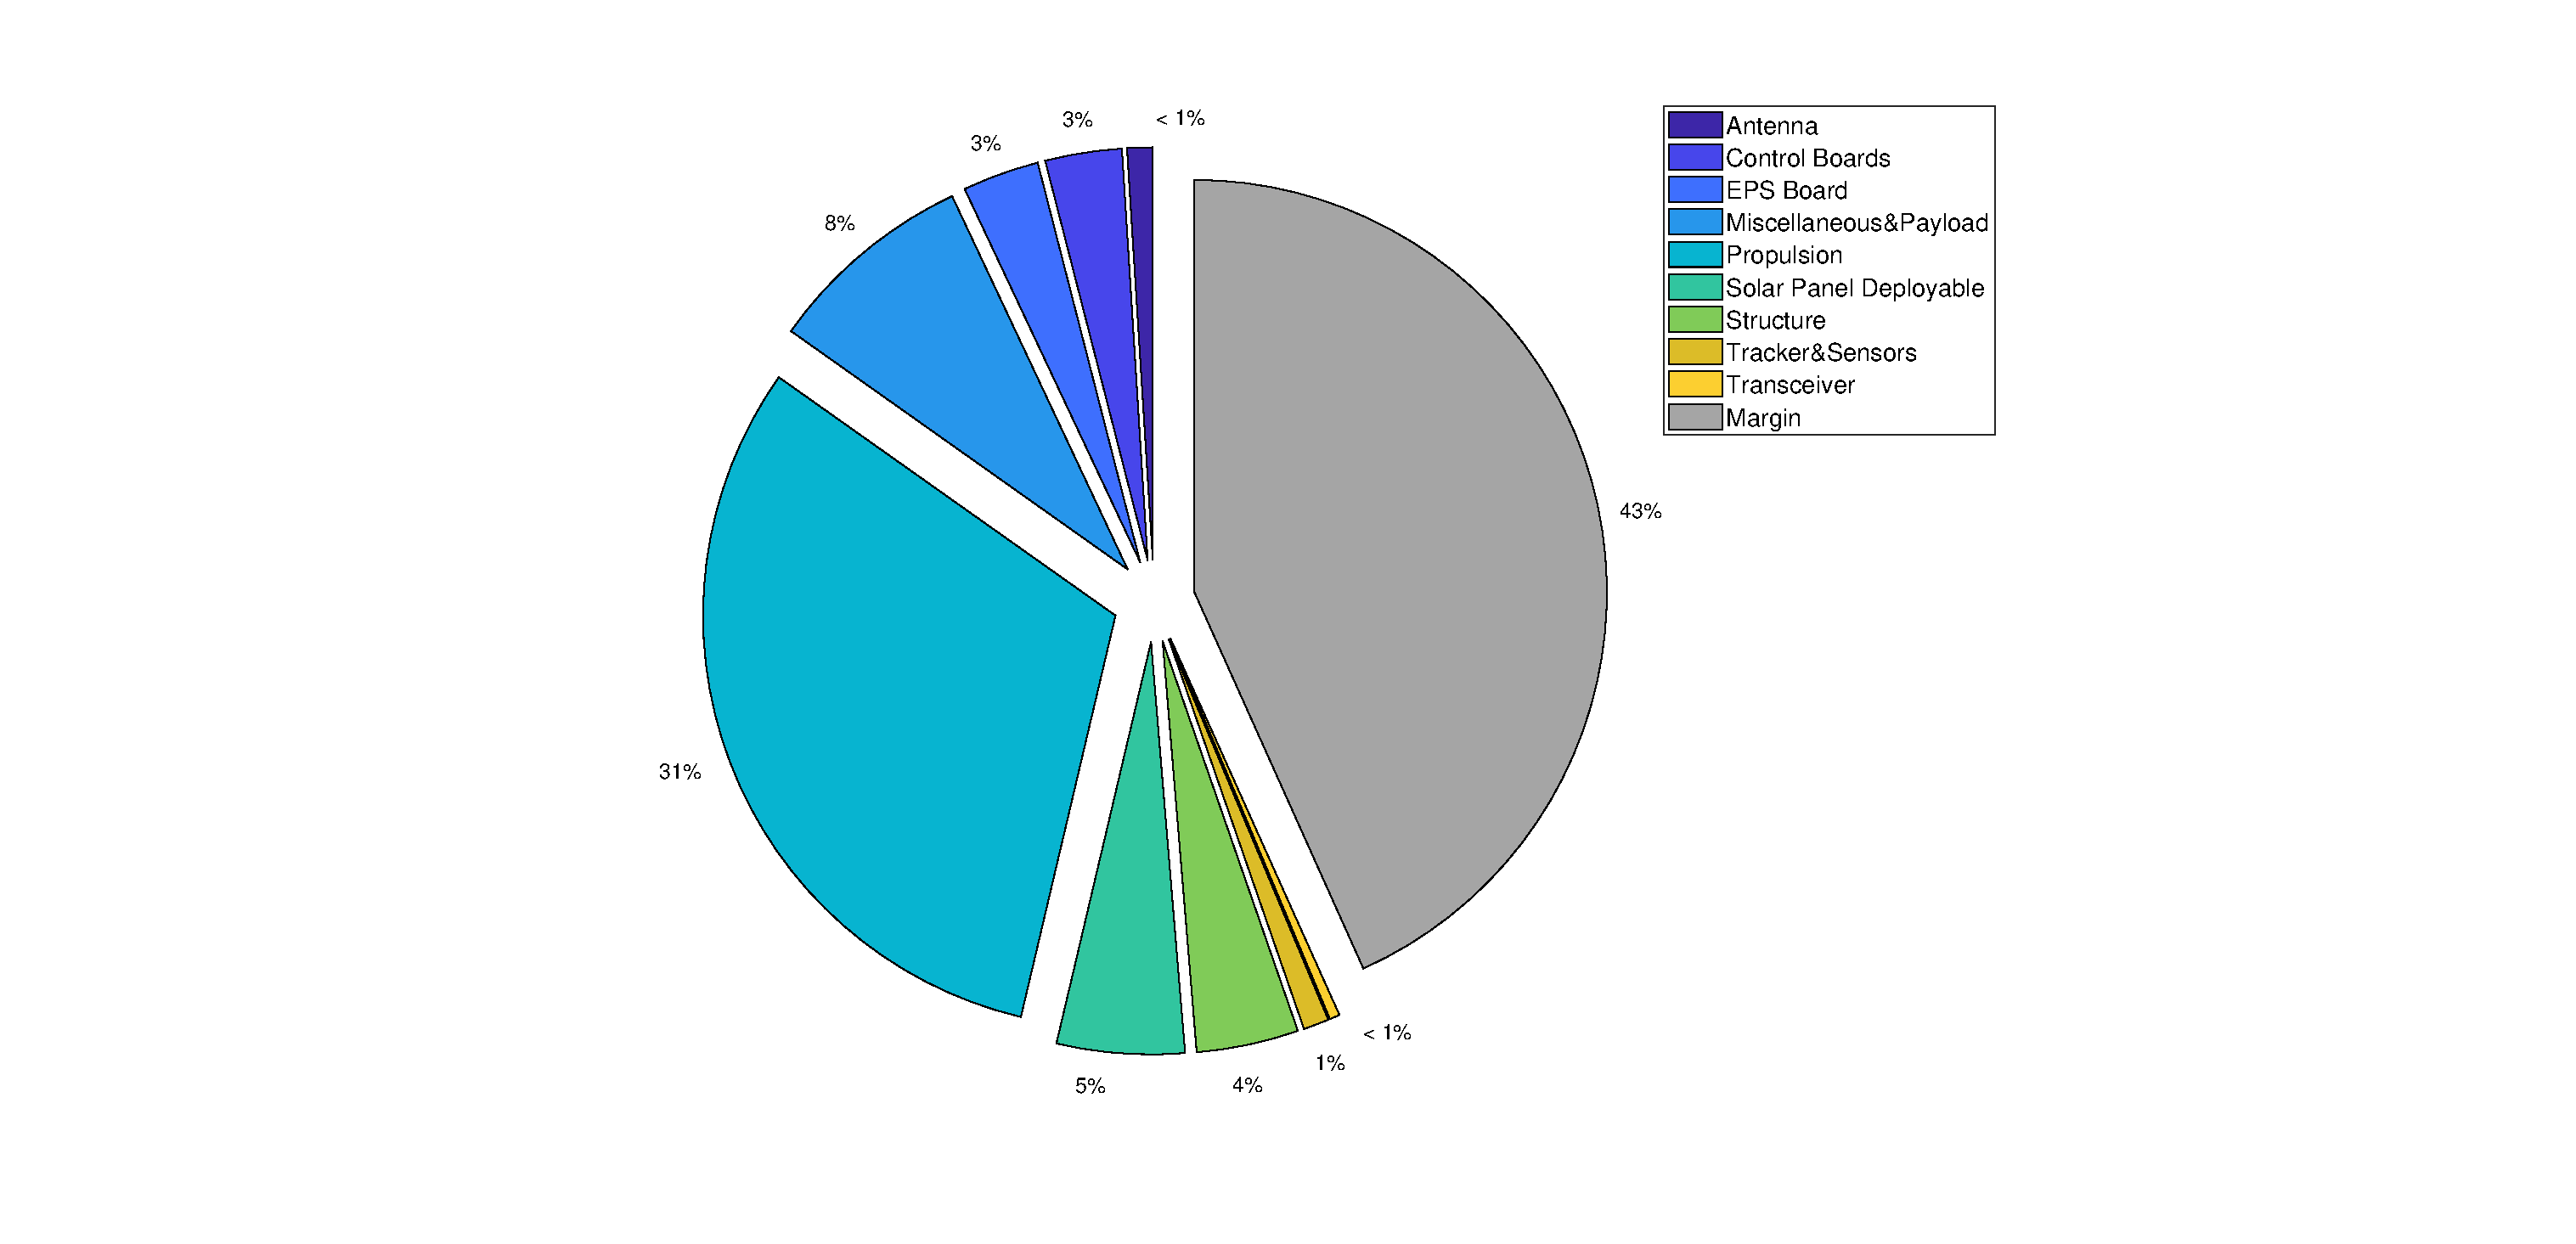
\includegraphics[width=1.00\textwidth]{masse}
											\caption{Massen Budget mittels QuSAD erstellt}
											\label{fig:masse}
										\end{figure}
										
						\subsubsection{Volumenbudget}
								
										\begin{figure}[h]
											\centering
												\includegraphics[width=1.00\textwidth]{volume}
											\caption{Volumen Budget mittels QuSAD erstellt }
											\label{fig:volume}
										\end{figure}
								
						\subsubsection{Leistungsbudget}
						\subsubsection{Preisbudget}
				
				\subsection{Konfigurationsvergleich}
		Budgets nur Vergleichen (kein GMAT) \\
		Datenbank soll möglichst nicht nur um die einzelnen Kompenenten erweitert werden (ruhig auch andere Komponenete aus der Excel Tabelle in die Datenbank aufnehmen)
		
		\section{	Ausgewähltes Missionsdesign}
		Kurze Beschreibung uas Max's Arbeit
				
